\documentclass[10pt,a4paper]{scrartcl}
\PassOptionsToPackage{table}{xcolor}
\usepackage[utf8]{inputenc}
\usepackage[T1]{fontenc}
\usepackage[ngerman]{babel}
\usepackage{microtype, multicol, marginnote, bera, parskip}
\usepackage{listings, amsmath, amssymb, graphicx, tikz, epic}
\usepackage{stmaryrd} %for lightning arrow
\usepackage{pstricks, pst-node, pst-tree, pdflscape}
\usepackage[babel=true]{csquotes}
\usepackage{placeins}
\usepackage[labelformat=empty]{caption}
\tolerance=2000
\setcounter{secnumdepth}{0}
\usepackage[inner=2cm,outer=2cm,top=1.5cm,bottom=1.5cm,includeheadfoot]{geometry}
\usepackage{multirow}
\newcommand{\subExercise}[1]{\vspace{0.5em} \noindent{\bf #1)}}
\newcommand{\B}{\mathbb{B}}
\DeclareMathOperator{\op}{op}

\author{Michael Mardaus \and Andrey Tyukin}
\title{
\includegraphics[scale=0.2]{../logo_schriftzug}\\
Technische Informatik: Abgabe 8}

\begin{document}

\maketitle

\section*{Exercise 8.1 (JK Flipflop Ringcounter)}
@Andrey You wanted to try to get to that circuit, right? It should work out if you name the states naturally from 000 to 111.\\
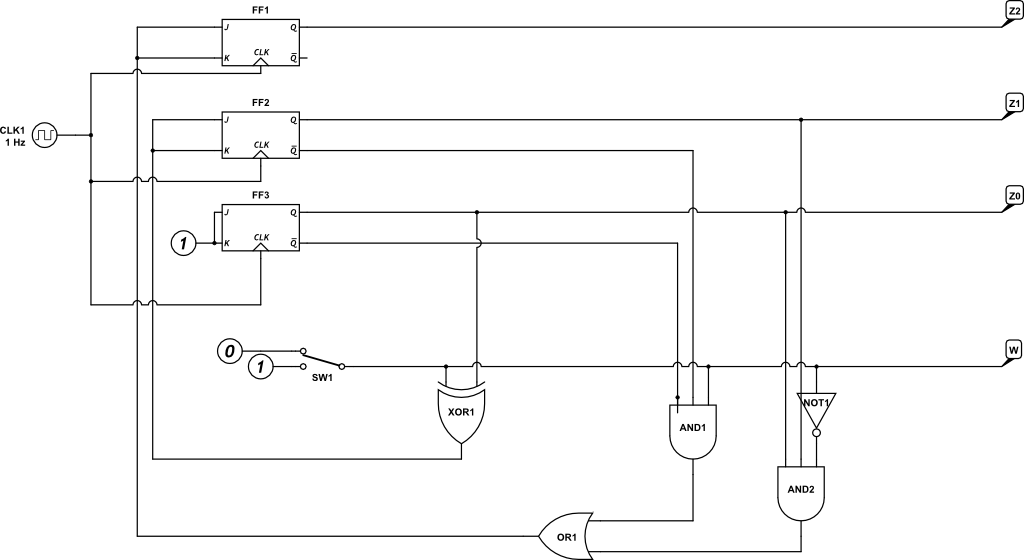
\includegraphics[width=\textwidth]{images/8_1-ringcounter-jk.png} 

\FloatBarrier
\section*{Exercise 8.2 (JK Flipflip for 4 equal inputs)}

First we make one input signal $w$ out of the $w_1$ and $w_2$ to make the automaton simpler. Therefore we XOR the two signals to one.
If both signals are equal XOR makes $w=0$. If they are different XOR will be $w=1$.\\
The state diagram for the automaton:

\begin{figure}[h]
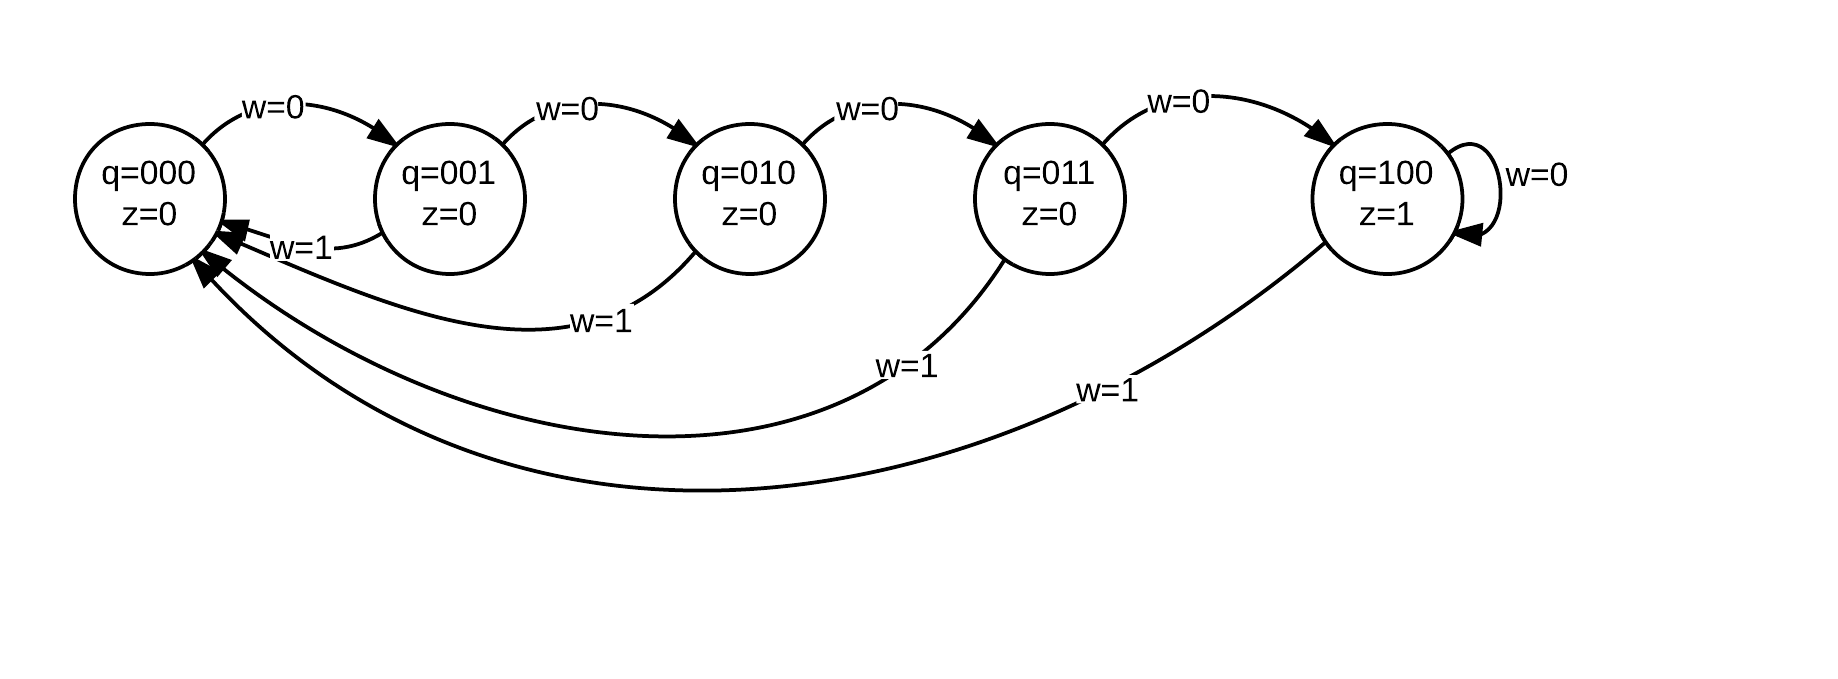
\includegraphics[width=\textwidth]{images/8_2-automat.png} 
\end{figure}

\begin{tabular}{|c||c|c|c|c||c|c|c|c||c|}

  \hline
  State     & \multicolumn{8}{c||}{Next state}             & \multicolumn{1}{c|}{Output} \\
            & \multicolumn{4}{c||}{$w=0$}                  & \multicolumn{4}{c||}{$w=1$}                  &  \\
$y_2y_1y_0$ & $Y_2Y_1Y_0$ & $J_2K_2$ & $J_1K_1$ & $J_0K_0$ & $Y_2Y_1Y_0$ & $J_2K_2$ & $J_1K_1$ & $J_0K_0$ & $z$  \\ \hline\hline
  000       & 001         & 0d       & 0d       & 1d       & 000         & 0d       & 0d       & 0d       & 0    \\ \hline  
  001       & 010         & 0d       & 1d       & d1       & 000         & 0d       & 0d       & d1       & 0    \\ \hline  
  010       & 011         & 0d       & d0       & 1d       & 000         & 0d       & d1       & 0d       & 0    \\ \hline  
  011       & 100         & 1d       & d1       & d1       & 000         & 0d       & d1       & d1       & 0    \\ \hline  
  100       & 100         & d0       & 0d       & 0d       & 000         & d1       & 0d       & 0d       & 1    \\ \hline \hline  
  101       & ddd         & dd       & dd       & dd       & 000         & dd       & dd       & dd       & d    \\ \hline  
  110       & ddd         & dd       & dd       & dd       & 000         & dd       & dd       & dd       & d    \\ \hline  
  111       & ddd         & dd       & dd       & dd       & 000         & dd       & dd       & dd       & d    \\ \hline  
\end{tabular}

This leads to these K-maps:\\
\begin{tabular}{|c||c|c|c|c|}
  \hline
 $J_0$   & \multicolumn{4}{c|}{$y_1y_0$} \\
  $wy_2$ & 00                 & 01                 & 11                 & 01                 \\ \hline\hline
  00     & \cellcolor{gray}1  & \cellcolor{gray}d  & \cellcolor{gray}d  & \cellcolor{gray}1  \\ \hline
  01     &                    & d                  & d                  & d                  \\ \hline
  11     &                    & d                  & d                  & d                  \\ \hline
  10     &                    & d                  & d                  &                    \\ \hline
\end{tabular}
\begin{tabular}{|c||c|c|c|c|}
  \hline
 $J_1$   & \multicolumn{4}{c|}{$y_1y_0$} \\
  $wy_2$ & 00                 & 01                 & 11                 & 01                 \\ \hline\hline
  00     &                    & \cellcolor{gray}1  & \cellcolor{gray}d  & d                  \\ \hline
  01     &                    & \cellcolor{gray}d  & \cellcolor{gray}d  & d                  \\ \hline
  11     &                    & d                  & d                  & d                  \\ \hline
  10     &                    &                    & d                  & d                  \\ \hline
\end{tabular}
\begin{tabular}{|c||c|c|c|c|}
  \hline
 $J_2$   & \multicolumn{4}{c|}{$y_1y_0$} \\
  $wy_2$ & 00                 & 01                 & 11                 & 01                 \\ \hline\hline
  00     &                    &                    & \cellcolor{gray}1  &                    \\ \hline
  01     & d                  & d                  & \cellcolor{gray}d  & d                  \\ \hline
  11     & d                  & d                  & d                  & d                  \\ \hline
  10     &                    &                    &                    &                    \\ \hline
\end{tabular}

\begin{tabular}{|c||c|c|c|c|}
  \hline
 $K_0$   & \multicolumn{4}{c|}{$y_1y_0$} \\
  $wy_2$ & 00                 & 01                 & 11                 & 01                 \\ \hline\hline
  00     & \cellcolor{gray}d  & \cellcolor{gray}1  & \cellcolor{gray}1  & \cellcolor{gray}d  \\ \hline
  01     & \cellcolor{gray}d  & \cellcolor{gray}d  & \cellcolor{gray}d  & \cellcolor{gray}d  \\ \hline
  11     & \cellcolor{gray}d  & \cellcolor{gray}d  & \cellcolor{gray}d  & \cellcolor{gray}d  \\ \hline
  10     & \cellcolor{gray}d  & \cellcolor{gray}1  & \cellcolor{gray}1  & \cellcolor{gray}d  \\ \hline
\end{tabular}
\begin{tabular}{|c||c|c|c|c|}
  \hline
 $K_1$   & \multicolumn{4}{c|}{$y_1y_0$} \\
  $wy_2$ & 00                 & 01                 & 11                 & 01                 \\ \hline\hline
  00     & d                  & \cellcolor{gray}d  & \cellcolor{gray}1  &                    \\ \hline
  01     & d                  & \cellcolor{gray}d  & \cellcolor{gray}d  & d                  \\ \hline
  11     & \cellcolor{gray}d  & \cellcolor{gray}d  & \cellcolor{gray}d  & \cellcolor{gray}d  \\ \hline
  10     & \cellcolor{gray}d  & \cellcolor{gray}d  & \cellcolor{gray}d  & \cellcolor{gray}1  \\ \hline
\end{tabular}
\begin{tabular}{|c||c|c|c|c|}
  \hline
 $K_2$   & \multicolumn{4}{c|}{$y_1y_0$} \\
  $wy_2$ & 00                 & 01                 & 11                 & 01                 \\ \hline\hline
  00     & d                  & d                  & d                  & d                  \\ \hline
  01     &                    & d                  & d                  & d                  \\ \hline
  11     & \cellcolor{gray}1  & \cellcolor{gray}d  & \cellcolor{gray}d  & \cellcolor{gray}d  \\ \hline
  10     & \cellcolor{gray}d  & \cellcolor{gray}d  & \cellcolor{gray}d  & \cellcolor{gray}d  \\ \hline
\end{tabular}

These K-maps lead us to:
\begin{eqnarray*}
    J_0 &=& \bar w\bar y_2\\
    J_1 &=& \bar wy_0\\
    J_2 &=& \bar wy_1y_0\\
    K_0 &=& 1\\
    K_1 &=& w+y_0\\
    K_2 &=& w
\end{eqnarray*}

Which brings us to this circuit:
\begin{figure}[h]
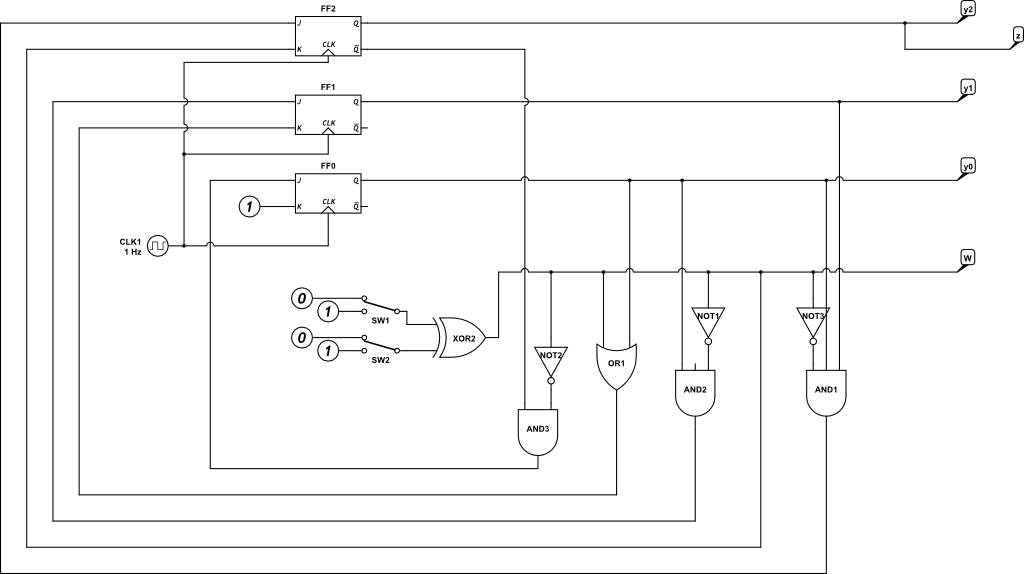
\includegraphics[width=\textwidth]{images/8_2-4counter.png} 
\end{figure}

\FloatBarrier
\section*{Exercise 8.3 (TODO)}

TODO Andrey?
\end{document}

